\documentclass{article}
\usepackage[a4paper,hmargin={2.4cm,2.4cm},vmargin={2.4cm,2.4cm}]{geometry}
\usepackage[pdftex]{hyperref}
\usepackage{soul}
\usepackage{graphicx}

\begin{document}
\title{Appendix 3: BBS Results}
\maketitle
\renewcommand*\thetable{S3.\arabic{table}}
\renewcommand*\thefigure{S3.\arabic{figure}}
\begin{table}[htb]
  \centering
  \small
\caption{Model selection table for ovenbirds in Maryland and Virginia,
    1966-2010.  We present model name and number, number of 
parameters (Par.), and difference in Akaike's
information criterion between each model and the top model of
that set ($\Delta$AIC).  The first section compares
models for initial abundance, the second for detection
probability, and the third for dynamics.}
  \begin{tabular}[h]{lcc}
\hline
Model	&Par.	&$\Delta$AIC	\\
\hline
A. Initial Abundance && \\
A.1. NB[$\Lambda$(.)$\alpha$(.)]Exponential[$r$(.)]$p$(.)	&4	&0\\
A.2. P[$\Lambda$(.)]Exponential[$r$(.)]$p$(.)	&3	&1262.7\\
A.3. ZIP[$\Lambda$(.)$\psi$(.)]Exponential[$r$(.)]$p$(.)	&4 &1264.7\\
\hline
B. Detection Probability && \\
B.1. NB[$\Lambda$(.)$\alpha$(.)]Exponential[$r$(.)]$p$(wind+1st)	&8 &0	\\
B.2. NB[$\Lambda$(.)$\alpha$(.)]Exponential[$r$(.)]$p$(wind) &7 &0.9\\
B.3. NB[$\Lambda$(.)$\alpha$(.)]Exponential[$r$(.)]$p$(1st)	&5	&5.0
\\B.4. NB[$\Lambda$(.)$\alpha$(.)]Exponential[$r$(.)]$p$(.)	&4	&6.4\\
\hline
C. Dynamics && \\
C.1. NB[$\Lambda$(.)$\alpha$(.)]Ricker-logistic+Immigration[$r$(.)$K$(.)$\iota$(.)]$p$(wind+1st) &10	&0	\\
C.2. NB[$\Lambda$(.)$\alpha$(.)]Gompertz-logistic+Immigration[$r$(.)$K$(.)$\iota$(.)]$p$(wind+1st) &10	&8.4 \\
C.3. NB[$\Lambda$(.)$\alpha$(.)]Exponential+Immigration[$r$(.)$\iota$(.)]$p$(wind+1st) &9	&36.5\\
C.4. NB[$\Lambda$(.)$\alpha$(.)]Geometric-recruitment+Immigration[$\gamma$(.)$\omega$(.)$\iota$(.)]$p$(wind+1st) &10	&38.6\\
C.5. NB[$\Lambda$(.)$\alpha$(.)]Gompertz-logistic[$r$(.)$K$(.)]$p$(wind+1st) &9	&192.8\\
C.6. NB[$\Lambda$(.)$\alpha$(.)]Ricker-logistic[$r$(.)$K$(.)]$p$(wind+1st) &9	&195.1\\
C.7. NB[$\Lambda$(.)$\alpha$(.)]Exponential[$r$(.)]$p$(wind+1st)	&8 &271.3\\
C.8. NB[$\Lambda$(.)$\alpha$(.)]Geometric-recruitment[$\gamma$(.)$\omega$(.)]$p$(wind+1st) &9	&273.7\\
C.9. NB[$\Lambda$(.)$\alpha$(.)]Constant-recruitment[$\gamma$(.)$\omega$(.)]$p$(wind+1st) &9	&1856.7\\
\hline
\end{tabular}
\end{table}
\clearpage

[Andy and Richard, which do you prefer for parameter estimates?  
Table or figure?  Either one may need a bit of work still.]
% latex table generated in R 3.0.0 by xtable 1.7-1 package
% Wed Sep 18 14:26:41 2013
\begin{table}[ht]
\centering
  \caption{Parameter estimates for ovenbirds in Maryland and Virginia from BBS data, 1966-2010.  
MLE estimates come from the NB[$\Lambda$(.)$\alpha$(.)]Ricker-logistic+Immigration[$r$(.)$K$(.)$\iota$(.)]$p$(wind+1st) 
model run in the \textbf{R} package \texttt{unmarked}; base estimates from the same model run in \textbf{JAGS};
obs estimates from the base model with random observer effects added; and ES estimates from the base
model with regional environmental stochasticity added.  Detectability parameters (intercept: $p_{0}$, 
effect of wind speed 1: $p_{1}$, effect of wind speed 2: $p_{2}$, effect of wind speed 3 or higher: $p_{3}$, 
effect of first run of a route by an observer: $p_{1st}$, and random observer effect: $\sigma_{p}$) are on the 
logit scale.}
\begin{tabular}{rllllll}
  \hline
 & Parameter & MLE & base & obs & ES & ES and obs \\ 
  \hline
1 & $\Lambda$ & 33.4 $\pm$ 4.7 & 31.1 $\pm$ 5.2 & 42.5 $\pm$ 7.3 & 33.2 $\pm$ 5.8 & 43.8 $\pm$ 7.9 \\ 
  2 & $\alpha$ & 0.654 $\pm$ 0.087 & 0.624 $\pm$ 0.108 & 0.730 $\pm$ 0.119 & 0.649 $\pm$ 0.110 & 0.753 $\pm$ 0.124 \\ 
  3 & $r$ & 0.026 $\pm$ 0.006 & 0.011 $\pm$ 0.005 & 0.018 $\pm$ 0.006 & 0.020 $\pm$ 0.010 & 0.023 $\pm$ 0.010 \\ 
  4 & $K$ & 56.9 $\pm$ 9.4 & 55.8 $\pm$ 18.2 & 101.8 $\pm$ 21.1 & 112.0 $\pm$ 58.8 & 141.5 $\pm$ 69.5 \\ 
  5 & $\iota$ & 0.283 $\pm$ 0.043 & 0.333 $\pm$ 0.043 & 0.306 $\pm$ 0.051 & 0.329 $\pm$ 0.046 & 0.303 $\pm$ 0.052 \\ 
  6 & $p_{0}$ & -1.492 $\pm$ 0.100 & -1.476 $\pm$ 0.097 & -1.994 $\pm$ 0.116 & -1.571 $\pm$ 0.099 & -2.056 $\pm$ 0.124 \\ 
  7 & $p_{1}$ & -0.012 $\pm$ 0.021 & -0.011 $\pm$ 0.021 & -0.014 $\pm$ 0.021 & -0.013 $\pm$ 0.021 & -0.015 $\pm$ 0.021 \\ 
  8 & $p_{2}$ & -0.075 $\pm$ 0.027 & -0.071 $\pm$ 0.027 & -0.056 $\pm$ 0.026 & -0.069 $\pm$ 0.027 & -0.055 $\pm$ 0.026 \\ 
  9 & $p_{3}$ & -0.133 $\pm$ 0.049 & -0.135 $\pm$ 0.049 & -0.145 $\pm$ 0.048 & -0.141 $\pm$ 0.049 & -0.144 $\pm$ 0.048 \\ 
  10 & $p_{1st}$ & -0.058 $\pm$ 0.028 & -0.047 $\pm$ 0.027 & -0.075 $\pm$ 0.029 & -0.045 $\pm$ 0.028 & -0.075 $\pm$ 0.029 \\ 
  31 & $\sigma_{p}$ & - & - & 0.353 $\pm$ 0.034 & - & 0.349 $\pm$ 0.034 \\ 
  42 & $\sigma_{\nu}$ & - & - & - & 0.074 $\pm$ 0.014 & 0.064 $\pm$ 0.014 \\ 
   \hline
\end{tabular}
\end{table}

\clearpage
\begin{figure}
  \centering
  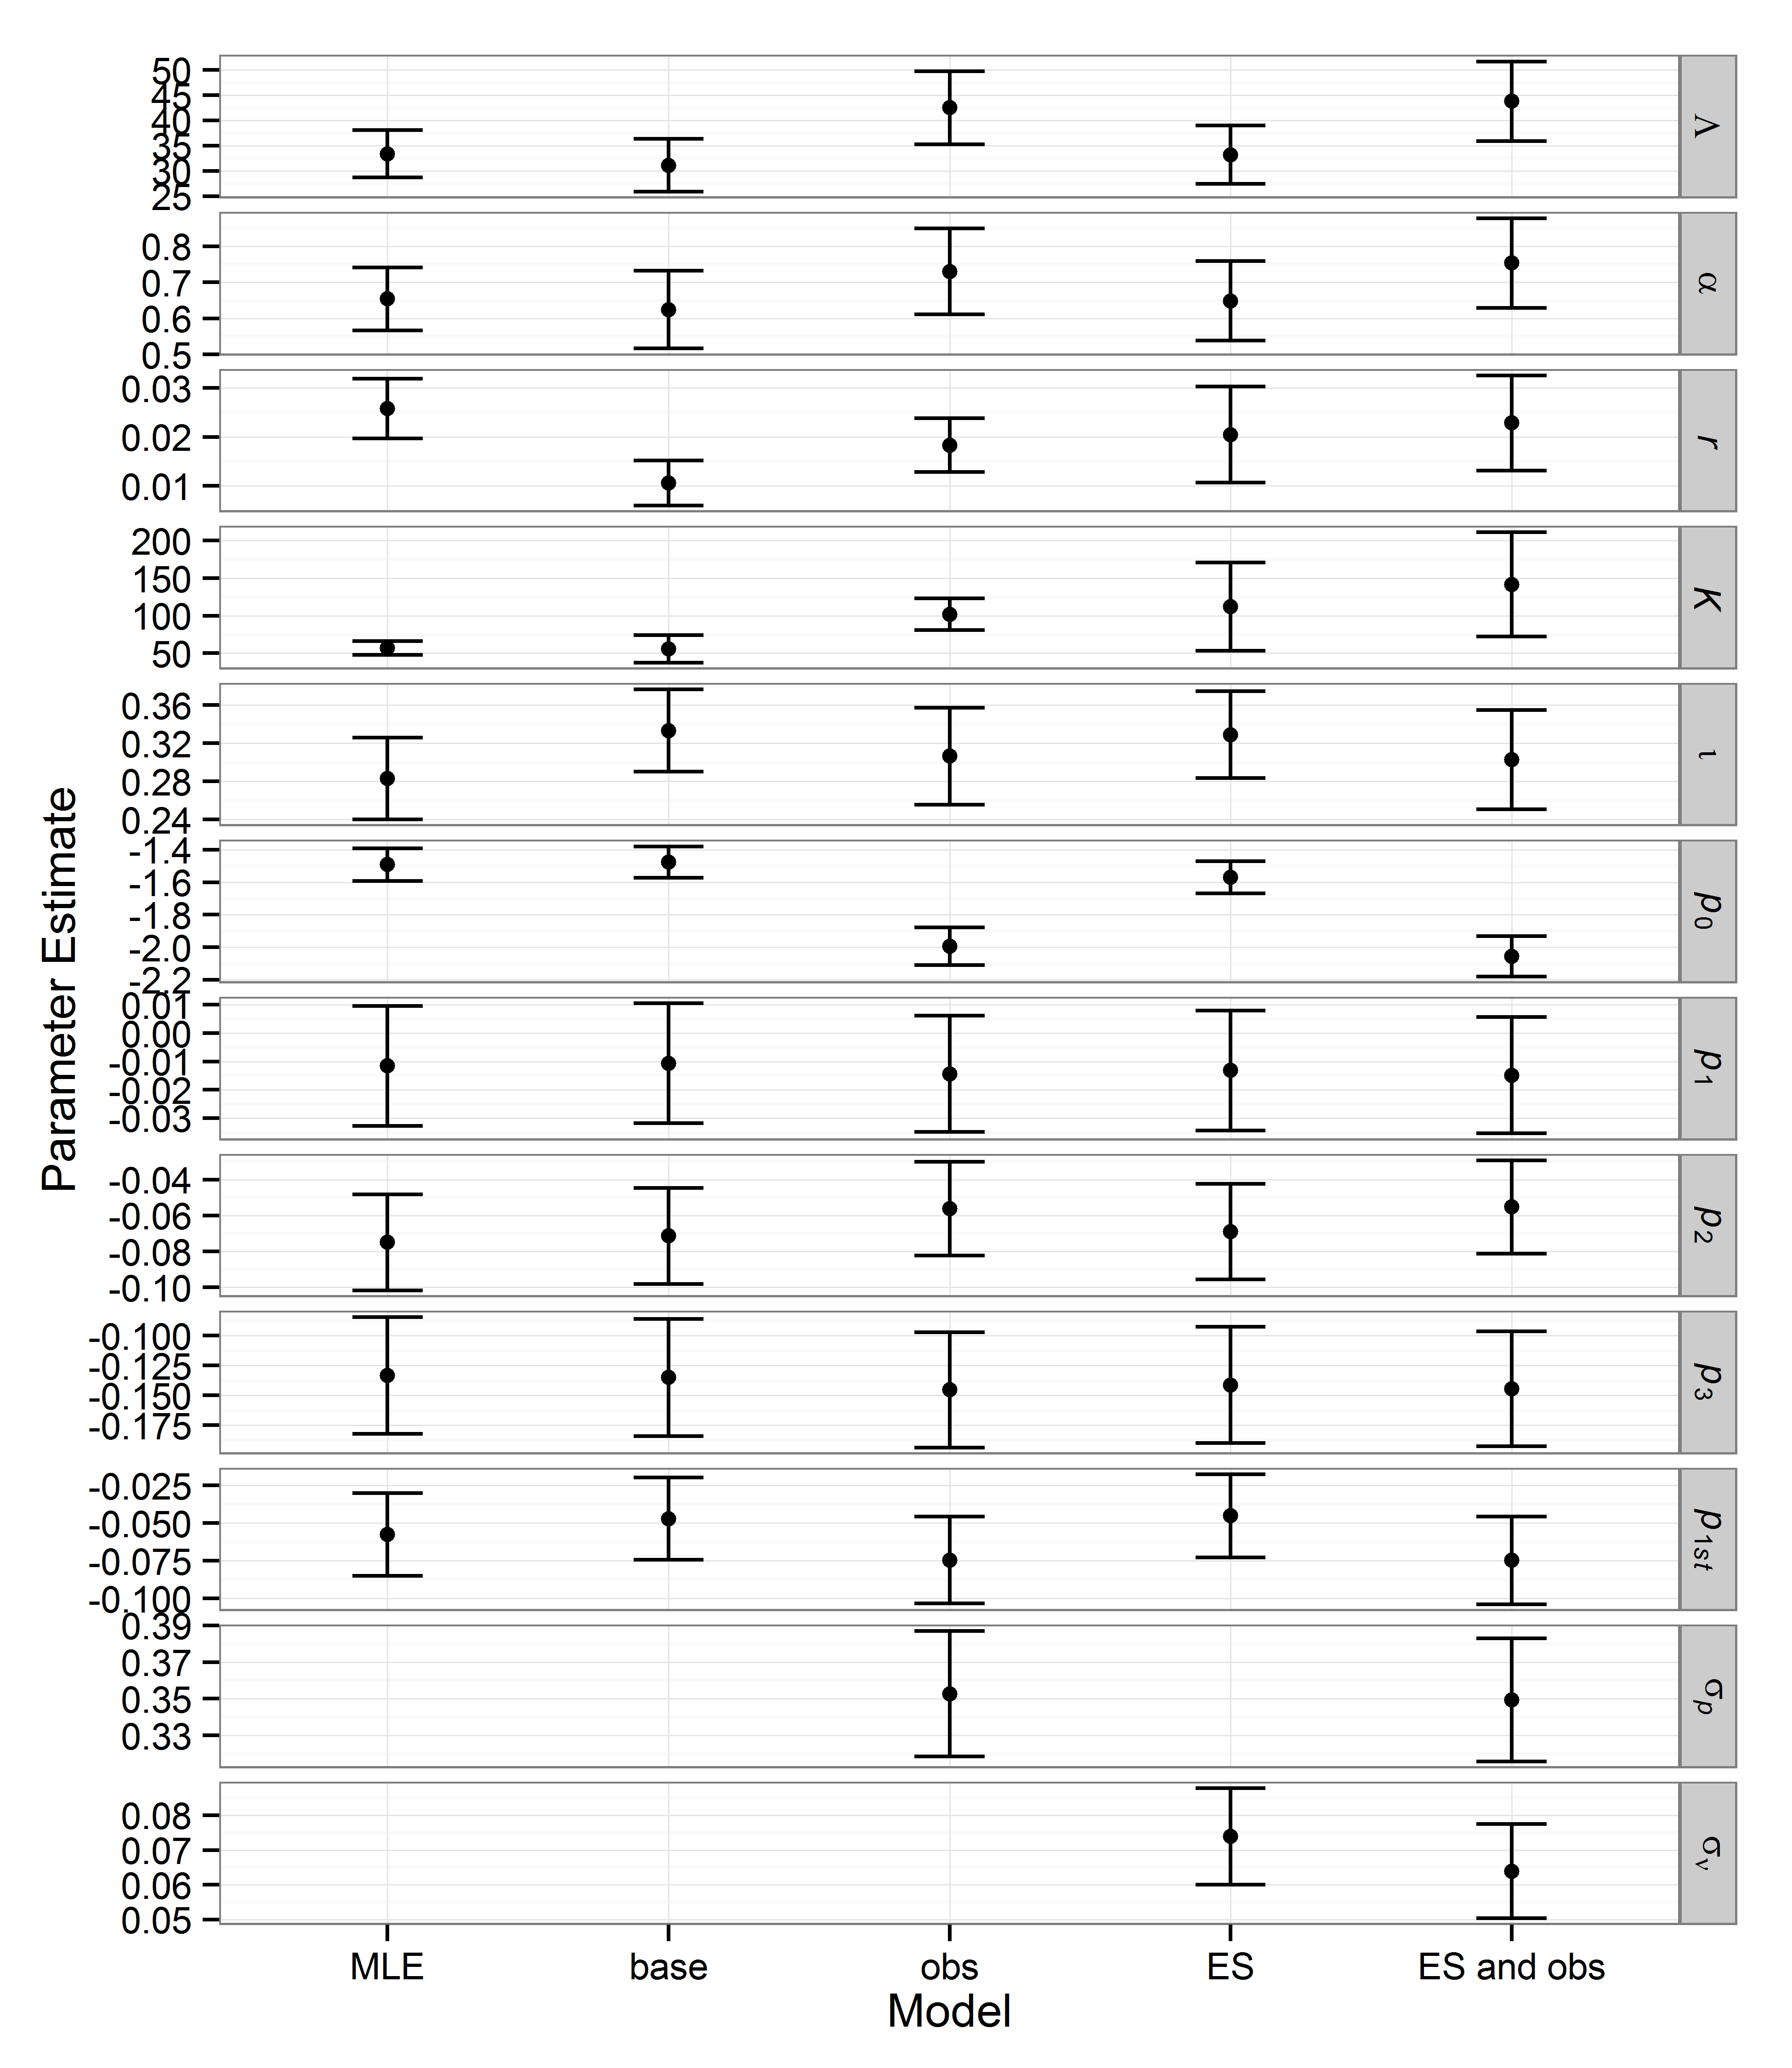
\includegraphics[width=6.5in]{../figs/oven_par_est}
\caption{Parameter estimates for ovenbirds in Maryland and Virginia from BBS data, 1966-2010.  
MLE estimates come from the NB[$\Lambda$(.)$\alpha$(.)]Ricker-logistic+Immigration[$r$(.)$K$(.)$\iota$(.)]$p$(wind+1st) 
model run in the \textbf{R} package \texttt{unmarked}; base estimates from the same model run in \textbf{JAGS};
obs estimates from the base model with random observer effects added; and ES estimates from the base
model with regional environmental stochasticity added.  Detectability parameters (intercept: $p_{0}$, 
effect of wind speed 1: $p_{1}$, effect of wind speed 2: $p_{2}$, effect of wind speed 3 or higher: $p_{3}$, 
effect of first run of a route by an observer: $p_{1st}$, and random observer effect: $\sigma_{p}$) are on the 
logit scale.}
\label{fig:oven_par_est}
\end{figure}


\end{document}
